\documentclass[a4paper, oneside]{book}

\usepackage{systeme, amsfonts, amsthm}
\usepackage[intlimits]{amsmath}
\usepackage{cancel}

\DeclareMathOperator*{\argmax}{arg\,max}
\DeclareMathOperator*{\argmin}{arg\,min}

% -- Настройка боковых заметок ------------------------------------------------
\usepackage[a4paper, marginparwidth=6cm, marginparsep=0.8cm]{geometry}
\geometry{left=1.5cm}
\geometry{right=8cm}

\setlength{\marginparpush}{15pt}


\usepackage[T2A]{fontenc} % Use 8-bit encoding that has 256 glyphs
\usepackage[utf8]{inputenc} % Required for including letters with accents
\usepackage[russian]{babel}
\usepackage{graphicx}
\graphicspath{{\subfix{pics/}}}

% marginnote создает НЕ нумерованные плавающие боковые заметки
\usepackage{marginnote}
\renewcommand*{\marginfont}{\footnotesize}

% Здесь делаем маленький шрифт для marginnote
\let\oldmarginpar\marginpar
\renewcommand\marginpar[1]{\-\oldmarginpar[\raggedleft\footnotesize #1]%
{\raggedright\footnotesize #1}}

% sidenotes создает НУМЕРОВАННЫЕ плавающие боковые заметки и боковые картинки
\usepackage{sidenotes}
% Здесь делаем маленький шрифт для sidenotes
\makeatletter
\RenewDocumentCommand\sidenotetext{ o o +m }{%      
    \IfNoValueOrEmptyTF{#1}{%
        \@sidenotes@placemarginal{#2}{\textsuperscript{\thesidenote}{}~\footnotesize#3}%
        \refstepcounter{sidenote}%
    }{%
        \@sidenotes@placemarginal{#2}{\textsuperscript{#1}~#3}%
    }%
}
\makeatother
% -----------------------------------------------------------------------------

% -- Настройка библиографии ---------------------------------------------------
\usepackage[backend=biber]{biblatex}
\addbibresource{biblio.bib}
% -----------------------------------------------------------------------------

\newtheorem{theorem}{Theorem}

\usepackage[breaklinks,hidelinks]{hyperref}
\usepackage{subfiles}

\title{\Huge{$\delta\alpha\alpha'$}: \\ Математика для анализа данных }

\author{Nurlan Sadykov}

% Абстракт
% Заметки по решению кубика рубика с помощью теории групп.

\begin{document}

\maketitle  
\tableofcontents


\part{Probability}

\section{Полная вероятность}
\marginpar{
    \begin{equation}
        \label{eq:low_of_full_probability}
        P(A) = \sum_i P(A|B_i) \cdot P(B_i)
    \end{equation}
}
Формула полной вероятности показывается как считается вероятность события, если
это событие может случиться при различных условиях. Само по себе правило
обычное, но очень полезны мат.ожидания и дисперсия полной вероятности.

\subsection{Правило полного мат.ожидания}
\marginpar{
    \begin{equation}
        \label{eq:low_of_total_expectation}
        E\lbrack X \rbrack = E\lbrack E\lbrack X|Y \rbrack\rbrack
    \end{equation}
}
В формуле полного мат.ожидания~\ref{eq:low_of_total_expectation} величина~$E[X|Y]$ случайная по~$Y$, поэтому в правой части формулы под внешним мат.ожиданием лежит не константа.

Доказательство формулы, такое:
\begin{multline*}
E[E[X|Y]] = E\left[ \sum_x x P(X=x|Y)\right] = \\
    \sum_y \left[ \sum_x x \, P(X=x|Y)\right] p(Y=y) = 
    \sum_y \sum_x x P(X=x, Y=y) = \\
    \sum_x x \sum_y P(X=x, Y=y) = \sum_x x \, P(X=x) = E[X]
\end{multline*}

\subsection{Правило полной дисперсии}
\marginpar{
    \begin{equation}
        \label{eq:low_of_total_variance}
        Var\lbrack Y \rbrack = 
        E\lbrack Var\lbrack Y | X \rbrack \rbrack + Var\lbrack E\lbrack Y | X \rbrack \rbrack
    \end{equation}
}
Разложим мат.ожидание $E[Y^2]$ по формуле полного мат.ожидания~\ref{eq:low_of_total_expectation} используя свойство $E[Y^2] = Var[Y] + E[Y]^2$
\[ E[Y^2] = E\left[ E[Y^2 | X] \right] = E[Var[Y | X] + E[Y | X]^2]\]
Теперь если разложить дисперсию, получим
\begin{multline*}
    Var[Y] = E[Y^2] - E[Y]^2 = \\
    E\left[Var[Y|X]\right] + E\left[E[Y|X]^2\right] - E\left[E[Y|X]\right]^2 =  \\
    E[Var[Y | X]] + Var[E[Y | X]]
\end{multline*}

\paragraph{Дисперсия при стратификации.}
\marginpar{
    Пример 1: Заработная плата в стране. Стратификация по регионам.

    Пример 2: Рост подростков. Стратификация по возрасту и/или полу.
}
Предположим, $X$ имеет мультиномиальное распределение и принимает значения от~1 до~$K$. Обозначим соответствующие вероятности~$p_i$ для удобства. Мы хотим рассчитать вероятность величины~$Y$ которая зависит от~$X$.
\marginpar{
    $\mu_k$,~$\sigma_k$ --- параметры распределения~$Y$ внутри страты~$k$.
}
В формуле~\ref{eq:low_of_total_variance} участвует два слагаемых, которые можно вычислить напрямую
\begin{align*}
    E[Var[Y|X]] &= \sum_{k=1}^K \sigma_k^2 \, p_k, \\
    Var[E[Y | X]] &= \sum_{k=1}^K (\mu_k - \mu)^2 \, p_k.
\end{align*}
Откуда и получим
\begin{equation}
    \label{eq:var_strat}
    Var[Y] = \sum_{k=1}^K \sigma_k^2 \, p_k + \sum_{k=1}^K (\mu_k - \mu)^2 \, p_k
\end{equation}

\section{Комбинации случайных величин}
\marginpar{
    $\xi_1,\;\xi_2$ --- случайные величины
    \\ $f_{\xi_1,\xi_2}(x_1,\,x_2)$ --- плотность совместного распределения
}
Допустим есть функция $g\colon \mathbb{R}^2 \to \mathbb{R}$ и мы хотим найти комбинацию двух случайных величин $\xi_1$ и~$\xi_2$, то есть мы хотим узнать функцию распределения для случайной величины $\eta = g(\xi_1,\,\xi_2)$. Посчитать величину~$\eta$ можно через функцию распределения
\begin{equation}
    \label{eq:g_xi_xi}
    F_\eta(x) = P(g(\xi_1, \xi_2) < x) =
    \iint\limits_{g(x_1, x_2) < x} f_{\xi_1,\xi_2}(x_1,\, x_2)\, dx_1\,dx_2
\end{equation}

В случае если случайные величины~$\xi_1$ и~$\xi_2$ независимы и $g(x_1,x_2) = x_1 + x_2$ можно показать, что плотность суммы выражается в виде свертки плотностей
\begin{equation}
    \label{eq:variable_sum}
    f_{\xi_1 + \xi_2} (t) = \int\limits_{-\infty}^\infty f_{\xi_1}(u)\,f_{\xi_2}(t - u)\,du
\end{equation}

\section{Характеристические функции}

\marginpar{
    Свойства:
    \begin{itemize}
        \item $\varphi_{a + b\xi}(t) = e^{ita}\varphi_\xi(tb)$
        \item $\varphi_{\xi + \eta} = \varphi_\xi(t) \cdot \varphi_\eta(t)$
        \item $\varphi_\xi^{(k)}(0) = i^k M\left(\xi^k\right)$ - $k$-ый момент это $k$-ая производная функции в нуле
    \end{itemize}
}
\emph{Характеристической функцией} случайной величины~$\xi$ называется функция
\begin{equation}
    \label{eq:characteristic_function}
    \varphi_\xi(t) = M\left(e^{it\xi}\right) = \int\limits_{-\infty}^\infty e^{itx} f(x)\,dx
\end{equation}

Характеристические функции это преобразование Фурье для случайных величин и по функции можно всегда восстановить распределение применив обратное преобразование.

\chapter{Распределения}
\section{Распределение хи-квадрат $\chi^2$}
Пусть $\xi_1, \cdots, \xi_k$ - независимые, стандартизованные, нормально распределенные случайные величины.
\marginpar{Стандартизованный: $\mu=0$, $\sigma=1$.}
Величина
\begin{equation}
    \label{eq:chi_def}
    \chi^2_k = \xi_1^2 + \ldots + \xi_k^2
\end{equation}
подчиняется распределению $\chi^2_k$  с~$k$ степенями свободы.

Плотность распределения 
\begin{equation}
    \label{eq:chi_pdf}
    f_{\chi^2_k}(x) = \frac{1}{2^{k/2}\Gamma(k/2)} x^{k/2-1} e^{-x/2}
\end{equation}

\section{Распределение Фишера-Снедекора}
Положим есть две случайные величины $U$ и~$V$ распределенные по $\chi^2$ с $n$ и~$k$ степенями свободы соответственно. Величина
\[ F = \frac{U/n}{V/k} \]
имеет распределение Фишера-Снедекора.

Плотность распределения
\[
    f(x) = \left\{
        \begin{array}{lr}
            0, & x \leq 0 \\
            C_0 \frac{x^{n-2} / 2}{(k + n x)^{(n + k)/2}}, & x > 0
        \end{array}
    \right.
    \qquad
    C_0 = \frac{\Gamma(\frac{k+n}{2}) n^{n/2}k^{k/2}}{\Gamma(n/2) \Gamma(k/2)}
\]

\chapter{Большие числа}
\section{Закон больших чисел (Хинчина)}
\label{sec:low_of_large_number}
Есть последовательность независимых наблюдений $X_1,\;X_2,\;\cdots$ выбранных
из одного распределения с конечными мат.ожиданием~$\mu$ и
дисперсией~$\sigma^2$. Среднее значение выборки первых~$n$ элементов будет тоже
равно~$\mu$.
\marginpar{Неравенство Чебышева:
    \[ P(\mid x - \mu \mid\, \geq\, k \sigma) \,\leq\, \frac{1}{k^2} \]

}

\[
    m_n = \frac1n (X_1 + X_2 + \dots + X_n)
\]
\[
    M(m_n) = \frac1n (M(X_1) + M(X_2) + \dots + M(X_n))
    = \mu
\]
А еще можем посчитать дисперсию:
\begin{equation}
    \label{eq:var_dispersia}
    D(m_n) = \frac{1}{n^2} \left(
            D(X_1) + D(X_2) + \cdots + D(X_n)
        \right)
        =
        \frac{1}{n^2} n \sigma^2 = \frac{\sigma^2}{n}
\end{equation}

Тогда если воспользоваться неравенством Чебышева, получим
\[
    P\left(|m_n - \mu| \geq \epsilon\right) = 
    P\left(|m_n - \mu| \geq \epsilon \frac{\sqrt{n}}{\sigma} \frac{\sigma}{\sqrt{n}}\right) \leq 
    \frac{\sigma^2}{n\,\epsilon^2}
\]
\marginpar{
    \emph{Что все это значит!} ЗБЧ Хинчина говорит, что для больших выборок оценка мат.ожидания через среднее почти наверняка совпадет с истинным мат.ожиданием. С ростом объема выборки, вероятность совпадения стремится к~1.
}
Теперь можем посчитать вероятность малых различий в разности
\[
    P\left(|m_n - \mu| < \epsilon\right) = 
    1 - P\left(|m_n - \mu| \geq \epsilon \right) \geq 
    1 - \frac{\sigma^2}{n\,\epsilon^2}.
\]

Откуда можем вывести предел по вероятности
\begin{equation}
    \label{eq:LLN}
    \lim_{n \to \infty} m_n = \mu
\end{equation}

\section{Центральная предельная теорема}
\marginpar{
    $X_{i \geq 1}$ - произвольные случайные величины из одного распределения
    с мат.ожиданием~$\mu$ и дисперсией~$\sigma^2$.
}
В общем виде центральную предельную теорему можно выразить так: \emph{мат.ожидание выборки имеет нормальное распределение.}

Для z-score 
\[ z_n = \frac{\sqrt{n}}{\sigma}\left(m_n - \mu\right) \]
теорема выражается так
\begin{equation}
    \label{eq:CLT}
    \lim_{n \to \infty} P(z_n \leq z) = \frac{1}{\sqrt{2\pi}} \int_{- \infty}^z
    \exp^{-x^2 / 2}\,dx = \Phi(z).
\end{equation}
\marginpar{
Для биномиального распределения $\mu=p$ и $\sigma = \sqrt{pq}$ откуда $ 
    z_n = \frac{\sqrt{n}}{\sqrt{p(1-p)}}\left( \frac{k}{n} - p \right)
    = \frac{k - np}{\sqrt{np(1-p)}}
$
}


\part{Statistics}

\section{Ящик с усами}

\begin{marginfigure}
    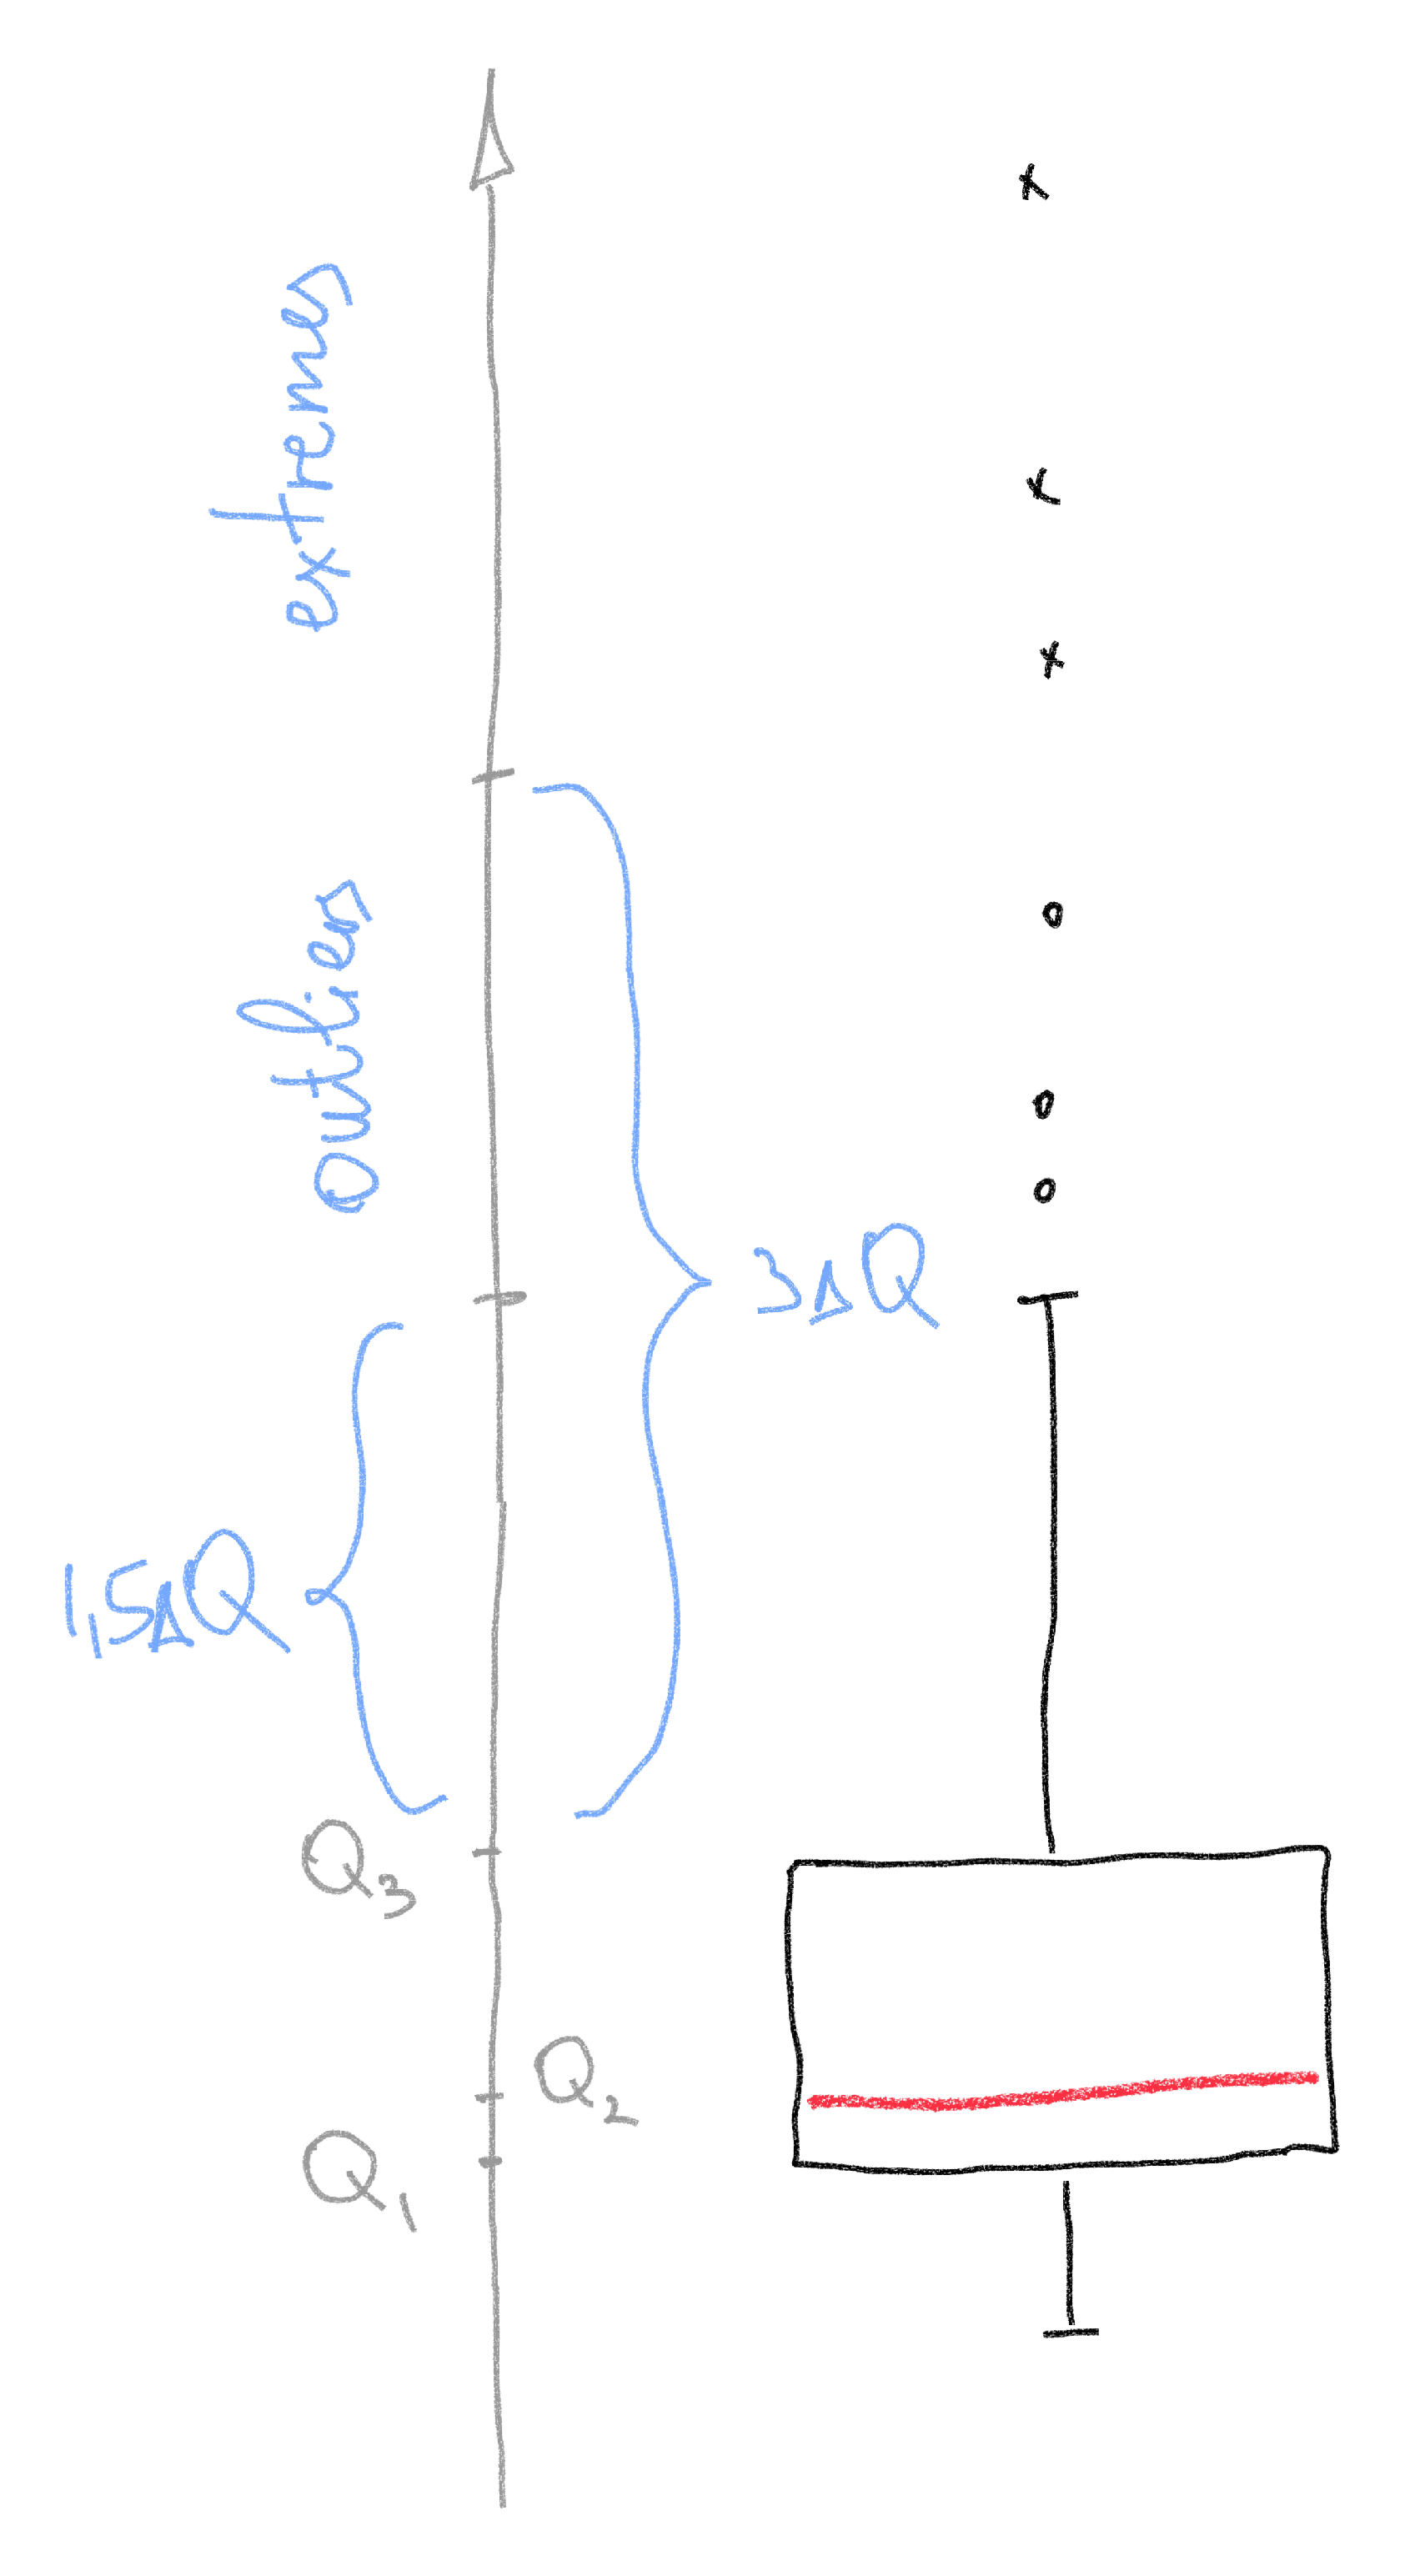
\includegraphics[width=0.7\columnwidth]{pics/boxplot.pdf}
    \label{fig:boxplot}
\end{marginfigure}

Есть набор наблюдений $x_1, \dots, x_n$, По набору можно вычислить:
\begin{itemize}
    \item $\min$ - минимальное наблюдение
    \item $\max$ - максимальное наблюдение
    \item $M$ - медиана
    \item $Q_1$ - первый квартиль (25\%)
    \item $Q_3$ - третий квартиль (75\%)
\end{itemize}

\emph{Межквартильный размах} задается разностью $\Delta Q = Q_3 - Q_1$.

Длина правого усика, это минимум между расстоянием от квартиля $Q_3$ до
максимального элемента и полутора полуторным межквартильным расстоянием.
Аналогично расчитывается длина правого усика.
\[l = \min(\max(x_i) - Q_3, 1.5 \Delta Q)\]
\[r = \min(Q_1 - \max(x_i), 1.5 \Delta Q)\]
Данные за усиками это \emph{выбросы}, а если они вышли за три межвартильных
расстояния это \emph{чрезвычайные выбросы}.

В ящике с усами используется медиана вместо матожидания
\marginpar{
    \emph{Усеченное среднее.} Если из выборки удалить 2,5\% самых маленьких
    наблюдений и 2,5\% самых больших, то выбросы уже не так сильно будут влиять
    на вычисленное матожидание.
}
в качестве описания потому, что она устойчива к
выбросам.

\subfile{statistica/ab_tests.tex}

\chapter{Статистические гипотезы. Базовые методы}

\section{Сравнение мат.ожиданий}
\marginpar{
    Для сравнения мат.ожиданий используются:
    \begin{itemize}
        \item t-критерий Стюдента
        \item Fligner-Killeen test
        \item Brown-Forsythe test
    \end{itemize}
}

При проверке гипотез часто встречаются понятия z-теста и t-теста. Оба теста имеют одни и те же формулы для расчета статистики, однако z-тест вычисляет критические точки из нормального распределения, а t-тест вычисляет критические точки из распределения Стьюдента.


\subsection{t-test, критерий Стьюдента}
Критерий Стюдента предполагает что метрика (н-р, матожидание) нормально распределена. Для двухвыборочного критерия важно равенство дисперсий. Так же тест не устойчив к выбросам в данных.

Одновыборочный тест\marginpar{
    Статистика для одновыборочного теста:\\
    $\overline x$ - выборочное матожидание \\
    $s^2$ - выборочная несмещенная оценка дисперсии \\
    $n$ - объем выборки
    \[H_0: M(x) = m\]
    \[t = \frac{\overline{x} - m}{s / \sqrt{n}}\]
    Степеней свободы $n-1$.
}
проводится когда у нас есть точное предположение о значении матожидания.

\paragraph{Двухвыборочный тест}
Предполагается, что есть две независимые выборки объема~$n_1$ и~$n_2$. Из
которых извлечены матожидания~$m_1$ и~$m_2$ и несмещенные дисперсии~$s_1^2$
и~$s_2^2$. 

\[H_0:m_1 = m_2\]

Если нулевая гипотеза верна, то разность $\Delta = m_1 - m_2$ имеет матожидание
$M(\Delta) = 0$\marginpar{
    Превращаем двувыборочный тест в одновыборочный!
}
и исходя из независимости выборок $D(\Delta) =
\frac{\sigma_1^2}{n_1} + \frac{\sigma_2^2}{n_2}$, так же получаем несмещенную
оценку разности выборочных средних $D(\Delta) = \frac{s_1^2}{n_1} +
\frac{s_2^2}{n_2}$. Теперь можем определить статистику

\begin{equation}
    \label{eq:t-test}
    t = \frac{m_1 - m_2}{\sqrt{\frac{s_1^2}{n_1} + \frac{s_2^2}{n_2}}}
\end{equation}

Степени свободы вычисляются по формуле
\begin{equation}
    \label{eq:t-test-degree}
    df = \frac{
        \left( \frac{s_1^2}{n_1} + \frac{s_2^2}{n_2}\right)^2
    }{
        (\frac{s_1^2}{n_1})^2/(n_1 - 1) + (\frac{s_2^2}{n_2})^2/(n_2-1)
    }
\end{equation}

\marginpar{
    Оценка показателей по выборке из генеральной совокупности всегда будет
    точечной оценкой. И если выбрать другую выборку, то оценка изменится. Чтобы
    учесть этот эффект вводят интервальную оценку показателя. 

    \vline

    \emph{Доверительный интервал} для показателя~$\nu$ это такой интервал
    $(\nu_l, \nu_r)$ в который истинный показатель входит с вероятностью $1 - \alpha$. 

}
\subsection{Доверительный интервал} Интервал строится исходя из препосылки, что распределение измерений матожиданий по различным выборкам из генеральной совокупности должно уложиться в нормальное распределение. Отсюда мы можем вычислить радиус доверительного интервала такими формулами
\begin{equation}
    \label{eq:m_confidence_interval}
    \Delta = \frac{s}{\sqrt{n}} \; z_\alpha
    \qquad\text{или}\qquad
    \Delta = \frac{s}{\sqrt{n}} \; t_\alpha(n-1)\;.
\end{equation}
Критерий выбирается исходя из количества наблюдений или каких-то других особенностей прода. Также вместо выборочного ср.кв.отклонения можно использовать и истинную дисперсию если она известна, как правило это большая редкость.

% Эту же формулу~\ref{eq:m_confidence_interval} можно использовать для вычисления
достаточного объема выборки. Если мы знаем максимальное расстояние которое
может достигать доверительный интервал, то остается только обернуть формулу.
Радиус подбирают таким, чтобы конкурирующая гипотеза не входила в интервал.


\subsection{Объем выборки}
\label{sec:sample_value}
\marginpar{
    $1 - \beta$ --- мощность (power) \\
    $\delta = m_1 - m_0$ --- MDE
}

Чтобы рассчитать объем необходимой выборки для проведения теста нужно зафиксировать уровень ошибок второго рода~$\beta$. Критическая точка определяет границу между принятием нулевой гипотезы или альтернативной. Если посчитать границу исходя из каждой гипотезы получим такое уравнение

\marginpar{
    \[
        z = \frac{x - m}{s}  \quad\longrightarrow\quad
        x = m + z \cdot s
    \]
}
\begin{equation}
    \label{eq:sample_size_border}
    \cancel{m_0} + z_{1-\alpha / 2} \,s_0 \sqrt{\frac{1}{n_0} + \frac{1}{n_1}}
    = 
    \cancel{m_0} + \delta - z_{1-\beta} \,\sqrt{\frac{s_0}{n_0} + \frac{s_1}{n_1}}.
\end{equation}

Уравнение~\ref{eq:sample_size_border} основа для расчета минимального объема выборки. Если предположить $n_0 = n_1 = n$, что обеспечит одинаковый объем в тестовом и контрольном сплитах, и $\sigma_0 = \sigma_1 = \sigma$ получим формулу
\marginpar{
    Chapter 2 in
    \fullcite{van2011statistical}
}
\begin{equation}
    \label{eq:sample_size_for_mean}
    n = 2\, \frac{s^2 (z_{1 - \alpha / 2} + z_{1 - \beta})^2}{\delta^2}
\end{equation}

\marginpar{
    Ср.кв.отклонение~$s$ обычно оценивают на исторических данных до эксперимента. Например средним значением за 5 месяцев.
}
Величина~$\delta$ определяет минимальный обнаруживаемый эффект MDE (minimal
detectable effect). В формуле~\eqref{eq:sample_size_for_mean} он присутствует в
виде делителя. Это значит, что за обнаружение минимального профита нам придется
заплатить увеличением выборки. 

\section{Сравнение медиан}
\marginpar{
Для сравнения медиан используются:
\begin{itemize}
    \item Mood's median test. Только для гигантских данных. На малых данных будет большая ошибка 2 рода.
    \item критерий Мана-Уитни. Есть критика критерия, но крайние случаи довольно редкие и ими пренебрегают и все равно используют критерий.
\end{itemize}
}

\subsection{Критерий Манна-Уитни. U-test.}

% \begin{marginfigure}
%     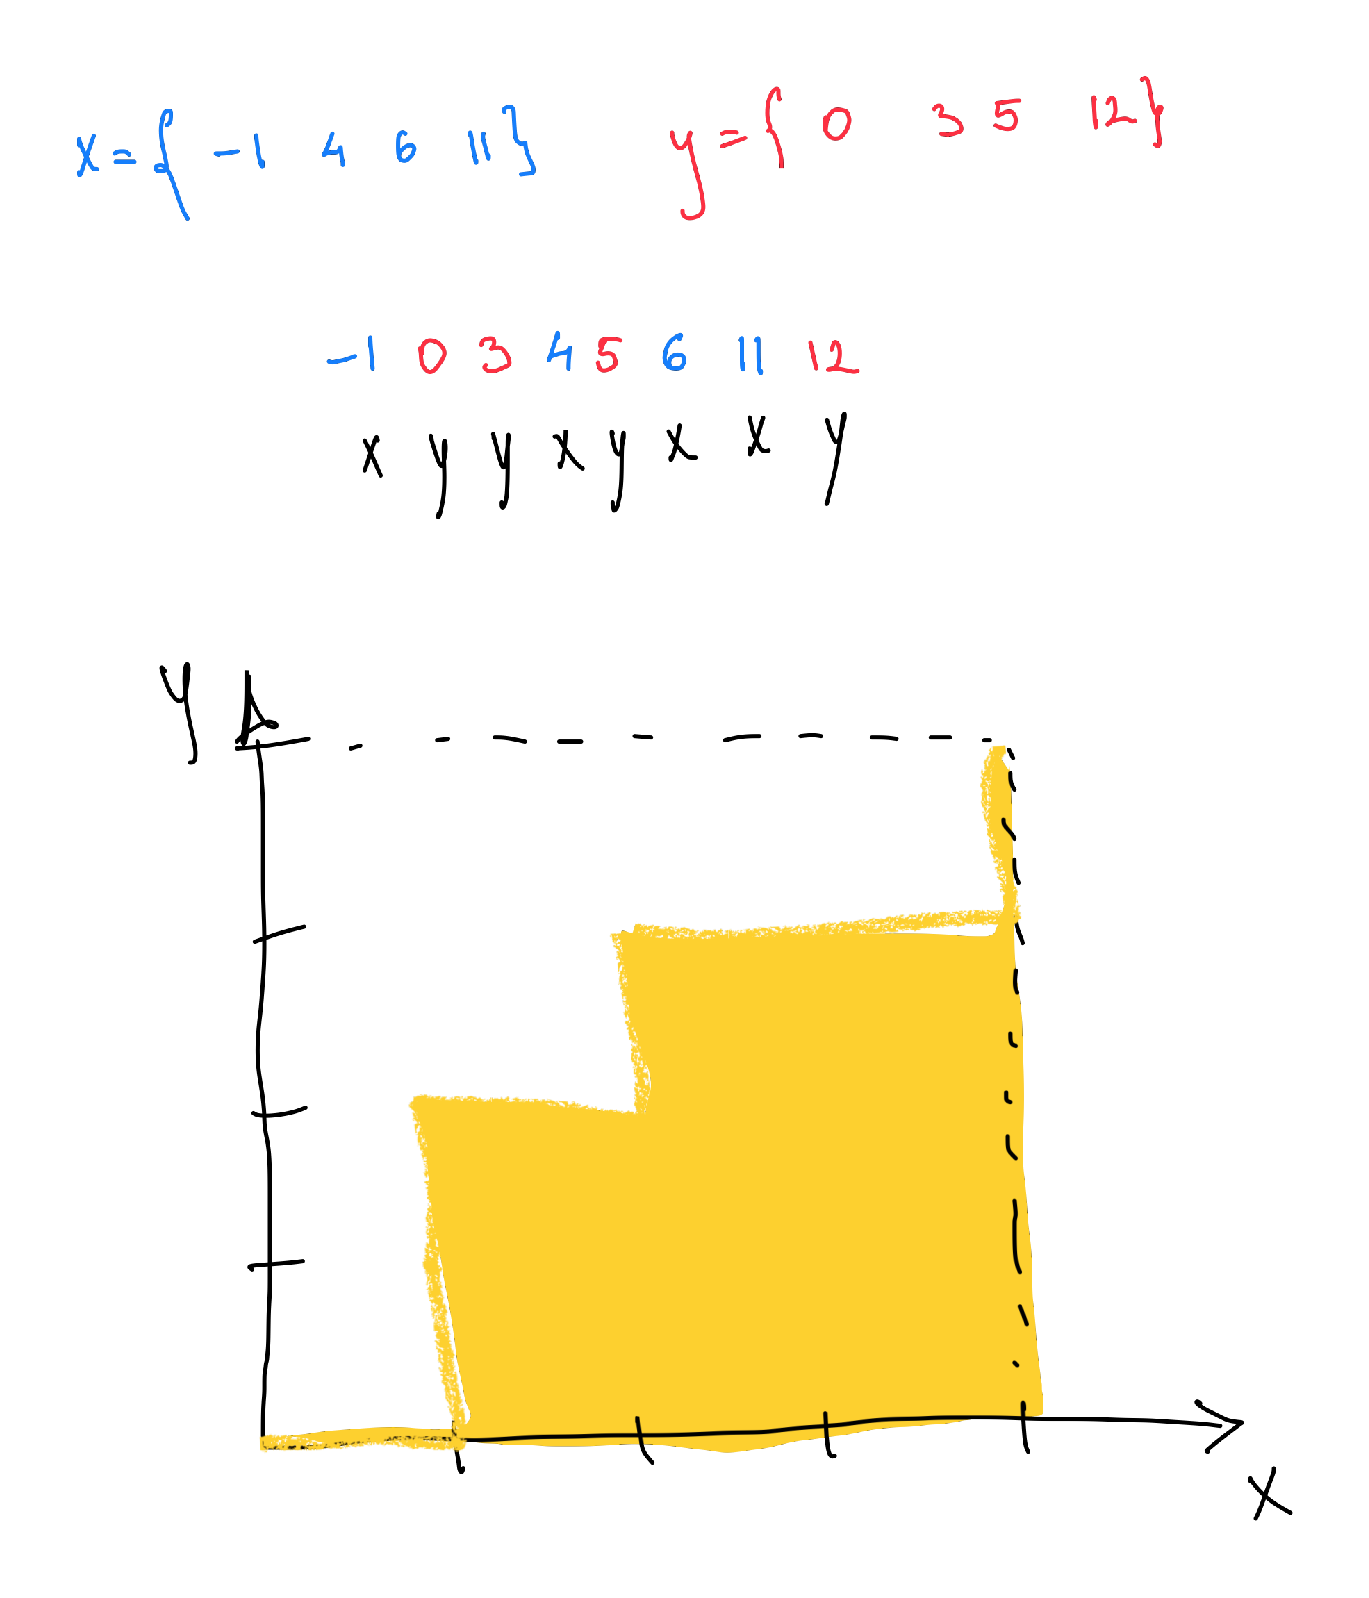
\includegraphics[width=1.1\columnwidth]{pics/mann-whitney_roc.pdf}
%     \label{fig:mann-whitney_roc}
% \end{marginfigure}
\begin{marginfigure}
    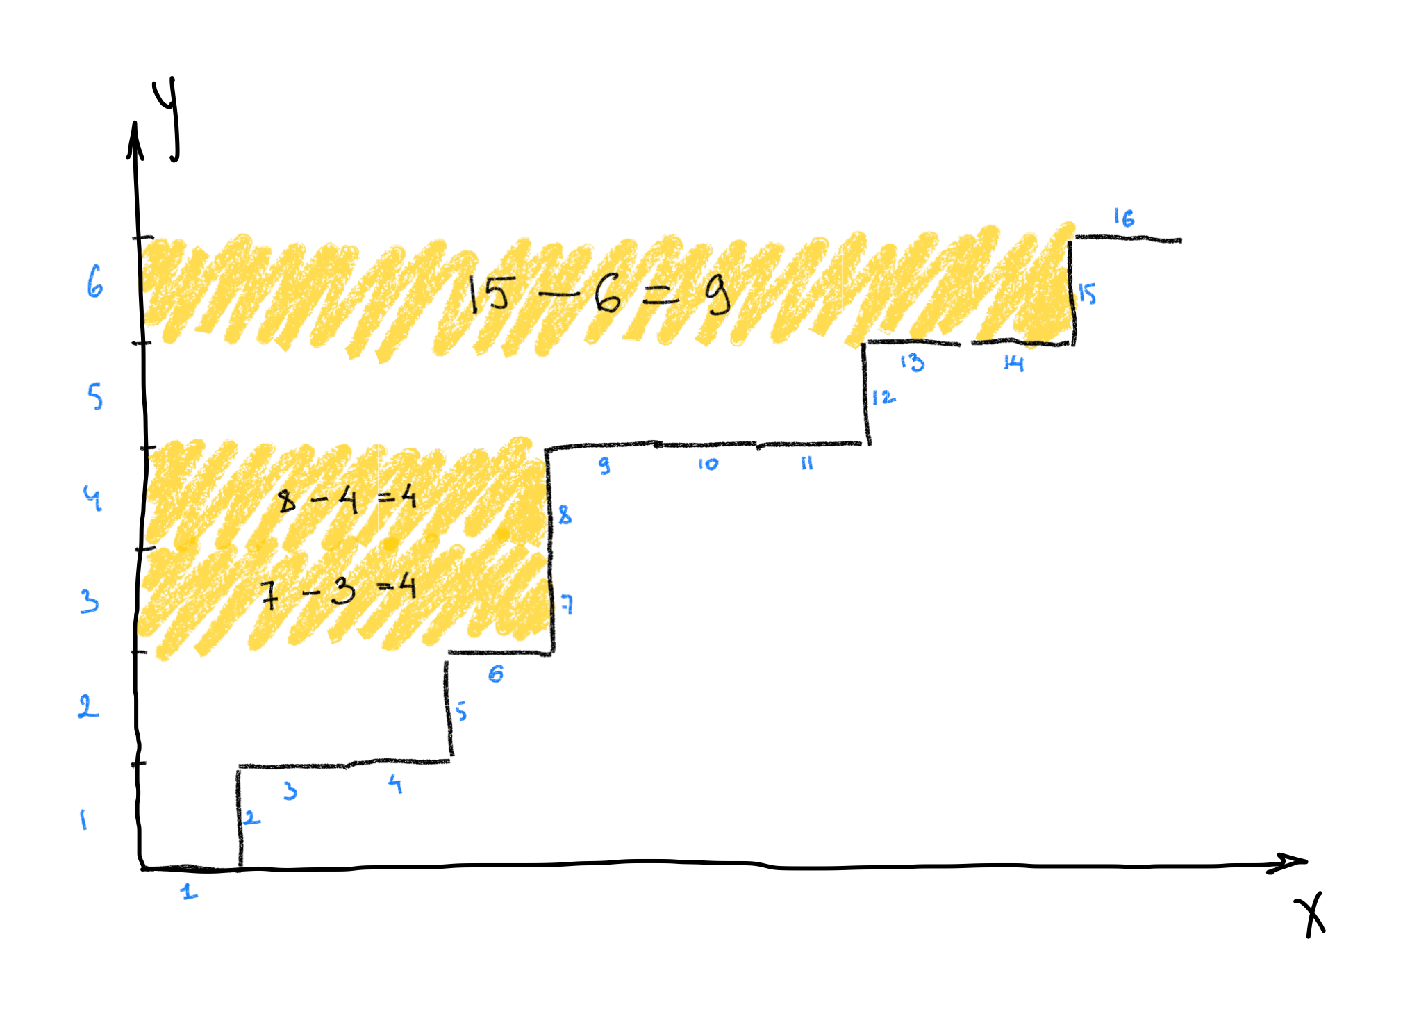
\includegraphics[width=1.1\columnwidth]{pics/Uy_square.pdf}
    \label{fig:mann-whitney_roc}
    \caption{
        Пояснение формулы $U_y$. По выборкам была составлена последовательность
        $XYXXYXYYXXXYXXYX$. Числа на ступенчатой кривой --- ранги в общей
        последовательности, числа на оси $Oy$ --- ранги в выборке~$y$.
    }
\end{marginfigure}
Чтобы применить критерий Манна-Уитни данные должны обладать порядком (числа
подходят). Это непараметрический тест поэтому область его применения может быть
шире, чем просто над числовыми показателями.

Положим есть две выборки $x_{i=\overline{1, n_1}}$ и~$y_{j=\overline{1, n_2}}$.
Тогда мы можем составить слово из букв~$X$ и~$Y$ последовательно вынимания из
объединения $x \cup y$ минимальный элемент. Буква определяется принадлежностью
множеству. Такую последовательность уже можно конвертировать в ROC кривую. Если
обе выборки принадлежат одному распределению, то буквы в слове перемешаются
равномерно, а значит кривая будет диагональю, площадь под которой равна
$S=\frac{n_1\,n_2}{2}$. Так мы свели задачу к проверки гипотезы о мат.ожидании.

\begin{itemize}
    \item[$H_0$:] Обе выборки из одной генеральной совокупности
    \item[$H_1$:] Выборки из разных генеральных совокупностей
\end{itemize}


Обозначим через $T_\ast$ сумму рангов элементов из разных выборок в объединении. Теперь мы можем посчитать
\begin{equation}
    \label{eq:Mann-Whitney:U}
    \left.
    \begin{array}{ll}
        U_x &= T_x - \frac{n_x (n_x + 1)}{2} \\
        U_y &= T_y - \frac{n_y (n_y + 1)}{2} \\
    \end{array}
    \;\right]
    \quad \Rightarrow \quad
    U = \min(U_x,\; U_y)
\end{equation}

\begin{equation}
    \label{eq:Mann-Whitney:z-value}
    \left.
    \begin{array}{ll}
        m_U &= n_x\,n_y / 2 \\ %\frac{n_x\,n_y}{2} \\
        s_U &= \sqrt{
            \frac{n_x\,n_y\,(n_x + n_y + 1)}{12}
        }
    \end{array}
    \;\right]
    \quad \Rightarrow \quad
    z = \frac{U - m_U}{s_U}
\end{equation}
\marginpar{\fullcite{watkins2019introduction}}

\paragraph{MDE} можно вычислять как для одновыборочного теста на мат.ожи\-да\-ние.

\section{Сравнение вероятностей (частот)}
\subsection{Классическая схема}
Количество появления события в выборке подчиняется биномиальному закону распределения $Bin(n, \pi)$
\marginpar{
    $n$ - количество испытаний \\
    $k$ - количество появлений события \\
    $\pi$ - \emph{истинная} вероятность события \\
    $p$ - \emph{оценка} вероятности (частоты)
}
При больших~$n$ биномиальное распределение становится близким к нормальному распределению с параметрами
\begin{equation}
    \label{eq:binomial2normal}
    m = p = \frac{k}{n} \qquad s = \sqrt{\frac{p (1 - p)}{n}}
\end{equation}
Задача снова сведена к сравнению через нормальное распределение. Значит можно воспользоваться z-тестом и z-статистика будет рассчитана так
\begin{equation}
    \label{eq:z-stat_for_prob}
    z = \frac{m_t - m_c}{\sqrt{\frac{s_t^2}{n_t} + \frac{s_c^2}{n_c}}}
\end{equation}

\subsection{Доверительный интервал}
\marginpar{
    Поскольку каждое изменение в выборке независимо, а объем выборки можно
    считать константой, можем сказать, что 
    \[ M[p\rbrack = M\lbrack k / n\rbrack  = M\lbrack k  / n\rbrack = np / n = p. \]
    Если учесть, что $ D\lbrack k \rbrack = npq $ и независимость выборки, получим
    \[ 
        D\lbrack p\rbrack =
        D\lbrack k / n\rbrack =
        D\lbrack k \rbrack / n^2 =
        npq / n^2 = pq / n.
    \]
}
Относительная частота события~$A$
вычисляется отношением $p = k / n$, где~$k$ --- число появлений события~$A$,
$n$ --- объем выборки. Тогда если учесть, что
\begin{equation}
    \label{eq:params_p_m_s}
    M[p] = p \qquad\text{и}\qquad D[p] = pq / n \,,
\end{equation}
можем воспользоваться формулой на вычисления вероятности интервала добавив еще уровень стат.значимости
\begin{equation}
    \label{eq:interval_prob_p}
    P(|X - k| < r) = 2\Phi(r / \sigma) = \alpha \,,
\end{equation}
откуда получим
\begin{equation}
    \label{eq:confidenc_interval_freq}
    r = z_\alpha \cdot \sqrt{\frac{p(1 - p)}{n}}
\end{equation}

Если нужно достать минимальный объем выборки, нужно знать заранее какой радиус~$r$ мы хотим обеспечить. Это можно определить исходя из потребности задачи (безнеса). Однако, есть еще один параметр который нужно знать заранее, это вероятность~$p$. Поскольку мы не знаем ее до эксперимента (получения выборки), можно положить $p = 0.5$. В этом случае выражение $p(1-p)$ примет наибольшее значение.

\subsection{Проверка гипотезы через beta-распределение}
\marginpar{
    Индекс $i = 0$ - контрольный сплит \\
    Индекс $i = 1$ - тестируемый сплит \\
    $k_i$ - наблюдаемые положительные эвенты \\
    $n_i$ - общий объем наблюдений \\
    $r_i = k_i / n_i$ - наблюдаемые доли \\
    $\rho_i$ - истинные доли
}

Если бы мы знали истинные доли в каждом из сплитов, то смогли бы рассчитать вероятность наблюдать~$k_i$ используя биномиальное распределение

\begin{equation}
    p(k_i | n_i, \rho_i) = Bin(n_i, \rho_i)
\end{equation}

Однако наша цель определить вероятность доли. Для этого воспользуемся формулой Байеса

\begin{equation}
    \label{eq:bayes_frequency}
    p(\rho_i = c | n_i, k_i) = \frac{p(k_i | n_i, \rho_i=c) p(\rho_i = c)}{
        \int_0^1 p(k_i | n_i, x) p(x) dx
    }
\end{equation}
Поскольку в качестве апостериорного распределения мы используем биномиальное, можем сразу указать априорное - beta-распределение. 

Причем вначале будем считать, что $k_i = 0$ и $n_i = 0$ при котором beta-распределение будет равномерным. 

\paragraph{p-value} вероятность наблюдать значение из тестируемого сплита (или хуже) при условии, что верна нулевая гипотеза. На формулах это будет выражено так
\[ p_{value} = \int_{k_1 / n_1}^1 Beta(x, k_0, n_0) dx \]

\paragraph{Доверительный интервал} задается через уровень статзначимости~$\alpha$ и формально может быть определен двумя уравнениями
\begin{align}
    \int_0^{r_l} Beta(x, k_i, n_i) dx &= \frac{\alpha}{2} \\
    \int_{r_r}^1 Beta(x, k_i, n_i) dx &= \frac{\alpha}{2}
\end{align}
\marginpar{В классической схеме интервал всегда получается симметричным.}
$r_l$ - левая граница интервала, $r_r$ - правая. Построенный таким образом интервал будет несимметричным, что бьется с тем, что частота всегда должна лежать в интервале $[0,\; 1]$ потому, что в противном случае мы бы вышли за пределы интервала.

\paragraph{MDE.} В классическое схеме используется трюк в котором любое
нормальное распреление можно масштабировать в стандартное простым линейным
преобразованием. К сожалению, для beta-распределения такого трюка нет и
придется все вычисления проводить напрямую. Воспользуемся идей из формулы~\ref{eq:sample_size_border}, то есть при фиксированных значениях~$\alpha$ и~$\beta$ вычислить минимальное $\delta$ при котором выполняется

\begin{equation*}
    \label{eq:beta_freq_mde}
    \left\{
    \begin{array}{cc}
        \int_{r_i + \delta}^1 Beta(x, k_0, n_0) \,dx &= \alpha \\
        \int_0^{r_i + \delta} Beta(x, k_1, n_1) \,dx &= \beta
    \end{array}
    \right.
\end{equation*}

\section{Исследование дисперсии}
\marginpar{
    $\mu,\;\sigma^2$ --- истинные мат.ожидание и дисперсия \\
    $m,\;s^2$ --- выборочные мат.ожидание и дисперсия
}
Предположим имеется выборка $x_1, \ldots, x_n \sim N(\mu, \sigma^2)$. Для исследования дисперсии выбирается одна из статистик в зависимости от того, что мы знаем о выборке.

\marginpar{
    См. следствия из леммы Фишера в
    \fullcite{cher2003_lectures}
}
\begin{itemize}
    \item При \emph{известном} мат.ожидании считаем величину 
        \begin{equation}
            \label{eq:chi_h_stat_mu}
            H = \sum_{i=1}^n\left(\frac{x_i - \mu}{\sigma^2}\right)^2
        \end{equation} 
        которая подчинена распределению $\chi^2_n$ c~$n$-степенями свободы.
    \item При \emph{неизвестном} мат.ожидании считаем величину
        \begin{equation}
            \label{eq:chi_h_stat_m}
            H = \sum_{i=1}^n\left(\frac{x_i - \mu}{\sigma^2}\right)^2 = \frac{(n-1)s^2}{\sigma^2}
        \end{equation} 
        которая имеет распределение $\chi^2_{n-1}$ с $(n-1)$-степенью свободы.
\end{itemize}

\subsection{Доверительный интервал}
\marginpar{
    $q_\psi$ - $\psi$-квантиль распределения~$\chi^2$ 
}
Поскольку мы знаем распределение статистики~$H$, можем определить границы в которых выполняется условие $P(q_{\alpha/2} < H < q_{1 - \alpha/2}) = 1 - \alpha$ и использовать их для определения доверительного интервала для дисперсии.

Например, при неизвестном мат.ожидании
\marginpar{
    Обрати внимание, что левый квантиль определяет правую границу, а правый квантиль - левую.
}
\[
    1 - \alpha = P\left(q_{\alpha/2} < \frac{(n-1)s^2}{\sigma^2} < q_{1 - \alpha/2}\right) =
    P\left(\frac{(n-1)s^2}{q_{1 - \alpha/2}}< \sigma^2 < \frac{(n-1)s^2}{q_{\alpha/2}} \right)
\]
остается только посчитать квантили $q_{1 - \alpha/2}$ и $q_{\alpha/2}$ и подставить в формулу.

\subsection{Гипотеза о числовом значении дисперсии}

\marginpar{
    Простая гипотеза:
    \begin{equation*}
        \left\{
            \begin{aligned}
                H_0: & \;\sigma = \sigma_0 \\
                H_1: & \;\sigma \ne \sigma_0
            \end{aligned}
        \right.
    \end{equation*}
}
В случае простой гипотезы, когда у нас есть предположение о значении дисперсии можно посчитать критические точки через интервальную оценку. Однако, проще воспользоваться оценкой p-value
\begin{equation}
    \label{eq:disp_p_value_hi2}
    \begin{aligned}
        F &= \int_0^H f_{\chi^2}(x) dx \\
        p_{value} &= 2 \min \left\{ F, 1 - F  \right\}
    \end{aligned}
\end{equation}


\marginpar{Сложная гипотеза:
    \begin{equation*}
    \begin{aligned}
        x_1, \ldots, x_n &\sim N(\mu_1, \sigma_1) \\
        y_1, \ldots, y_k &\sim N(\mu_2, \sigma_2)
    \end{aligned}
    \quad
        \left\{
            \begin{aligned}
                H_0: & \;\sigma_1 = \sigma_2 \\
                H_1: & \;\sigma_1 \ne \sigma_2
            \end{aligned}
        \right.
    \end{equation*}
}
\subsection{Гомогенность дисперсии}
Предположим, что есть вторая выборка~$Y$ и мы хотим проверить, что в обеих выборках дисперсии одинаковы. Величина $F = s^2_x / s^2_y$ имеет распределение Фишера-Снедкора со степенями свободы $n-1$ и $k-1$.
\marginpar{
    $s^2_x$ --- исправленная дисперсия выборки~$X$ \\
    $s^2_y$ --- исправленная дисперсия выборки~$Y$
}
В случае если дисперсии равны, значение статистики~$F$ должно находиться в районе 1. Зная распределение можно вычислить критическую точку или посчитать p-value.


\section{ANOVA: Дисперсионный анализ}
\marginpar{ANOVA: ANalysis Of VAriance}
\marginpar{
    $q$ --- количество групп  \\
    $n_j$ --- количество наблюдений в группе~$j$ \\
    $y_{ij}$ --- $i$-ое наблюдение в группе~$j$\\
    $\mu_j$ --- мат.ожидание в группе $j$

    \[ n = \sum_{j=1}^q n_j \]
}

Тест предназначен для экспериментов когда имеется более чем 2 группы. ANOVA
проверяет, что все группы имеют одинаковое мат.ожи\-да\-ния. Альтернативой
будет наличие хотя бы одной пары в которой не совпадают мат.ожидания.
\begin{equation}
    \label{eq:anova_hyps}
    \begin{cases}
        H_0: &\text{для всех}\; j,\,k,\quad  \mu_j = \mu_k, \\
        H_1: &\text{есть пара}\; j,\,k, \quad \mu_j \ne \mu_k
    \end{cases}
\end{equation}

\marginpar{
    \begin{eqnarray*}
        \overline{y}_j &=& \frac{1}{n_j}\sum_{i=1}^{n_j} y_{ij} \\
        \overline{\overline{y}} &=& \frac1n \sum_{j=1}^q n_j \overline{y}_j
    \end{eqnarray*}
}
Построим общую сумму квадратов
\begin{equation}
    \label{eq:SS_total}
    SS_{total} = \sum_{j=1}^q\sum_{i=1}^{n_j}(y_{ij} - \overline{\overline{y}})
\end{equation}
и разложим ее не две составляющие
\begin{equation*}
    \sum_{i=1}^{n_j}(y_{ij} - \overline{\overline{y}})^2 =
    \sum_{i=1}^{n_j}(y_{ij} - \overline y)^2 + n_j(\overline y_j - \overline{\overline{y}})^2
    = (n_j - 1) s_j^2 + n_j(\overline y_j - \overline{\overline{y}})^2
\end{equation*}
Используя эти формулы сможем разложить $SS_{total}$ на сумму внутригрупповых отклонений и на межгрупповых отклонений
\begin{equation}
    SS_{total} = SS_{residual} + SS_{between}
\end{equation}
\marginpar{
    $SS_{residual}$ имеет $n - q$ степеней свободы \\
    $SS_{between}$ имеет $q - 1$ степеней свободы \\
}
\begin{equation}
    \label{eq:ss}
    SS_{residual} = \sum_{j=1}^q(n_j-1) s_j^2 \qquad
    SS_{between} = \sum_{j=1}^q n_j(\overline y_j - \overline{\overline{y}})^2
\end{equation}
Если мат.ожидания во всех группах действительно равны, то межгрупповые ошибки не отличаются от внутригрупповых ошибок, а значит статистика~$F$ подчинена распределению Фишера
\begin{equation}
    F = \frac{SS_{between} / (q -1)}{SS_{residual} / (n - q)} \,.
\end{equation}

\subsection{Метод контрастов}
\marginpar{
    \begin{flalign*}
        y = c_1 \overline y_1 + \ldots + c_q \overline y_q \\
        M(y) = c_1 \mu_1 + \ldots + c_q \mu_q \\
        D(y) = \frac{c_1^2 \sigma_1^2}{n_1} + \ldots + \frac{c_q^2 \sigma_q^2}{n_q}
    \end{flalign*}
    для формулы дисперсии смотри~\ref{eq:var_dispersia}
}
Если мы отвергли нулевую гипотезу~\ref{eq:anova_hyps} и есть пара групп с различными мат.ожиданиями, следующим шагом будет указать эту пару. Рассмотрим более общую задачу, предположим, что есть линейная зависимость между значениями~$\mu_j$, то есть существуют такие коэффициенты \emph{(и мы их знаем)}, что $\sum_{j=1}^q c_j \overline y_j = 0$. Например, мы можем проверять гипотезу, что $\mu_2 = \mu_3$, что эквивалентно $\mu_2 - \mu_3 = 0$. Можем сформировать нулевую гипотезу и альтернативу
\begin{equation}
    \label{eq:anova_hyps}
    \begin{cases}
        H_0: &\sum_{j=1}^q c_j \overline y_j = 0 \\
        H_1: &\sum_{j=1}^q c_j \overline y_j \ne 0
    \end{cases}
\end{equation}
Изначально, мы ничего не знаем про дисперсии в группах. Поэтому делаем предположение, что дисперсии одинаковы для всех групп $\sigma_1 = \ldots = \sigma_q$. Тогда нам нужна оценка внутригрупповых дисперсий
\begin{equation}
    s_{residual}^2 = SS_{residual} / (n - q)
\end{equation}
Тогда оценить гипотезу~$H_0$ мы можем используя доверительный интервал для мат.ожидания
\marginpar{
    Для подбора коэффициентов нужно привлекать внешние предположения о природе данных. Нельзя просто подобрать коэффициенты~$c_j$ исходя из выборки, поскольку в этом случае ничто не мешает подобрать коэффициенты при которых выборочные средние в линейной комбинации дадут точный ноль.
}
\begin{equation}
    y \pm t_{1-\alpha,\, n - q} \, s_{residual} 
    \sqrt{
        \sum_{j=1}^q \frac{c_j^2}{n_j}
    }.
\end{equation}
Если интервал не покрывает ноль, то нулевая гипотеза отвергается.

\section{Проверка зависимости}
\marginpar{
    При проверке зависимости между двумя случайными величинами используют
    коэффициенты корреляции:

    \begin{itemize}
        \setlength\itemsep{0em}
        \item Пирсона, если данные нормальные.
        \item Спирмена, в остальных случаях.
        \item Кендела, очень редко.
    \end{itemize}
}

При вычислении корреляций надо понимать, что они ищут только линейные зависимости, коэффициенты могут быть очень чувствительными к выбросам и иногда могут показывать ложную корреляцию, например, для монотонных временных рядов.

\section{CUPED}
\marginpar{\it \tiny Controlled-experiment Using Pre-Experiment Data} 
%--- метод увеличения чувствительности эксперимента за счет снижения дисперсии. Чтобы воспользоваться методом необходимо, чтобы была накоплена какая-то предварительная история из которой мы вытащим дополнительные данные о процессе.
\marginpar{
    \fullcite{microsoft_cuped}
}

\marginpar{
    $\qquad Y$ --- случайная величина \\
    $M(Y)$ --- среднее значение величины~$Y$ \\
    $\qquad n$ --- объем выборки \\
    $\qquad\overline Y$ --- выборочная оценка среднего \\
    $var(\overline Y) = var(Y) / n$
}

Предположим мы хотим отловить изменения в случайной величине~$Y$, но она обладает очень большой дисперсией. Высокая дисперсия увеличивает время эксперимента, следовательно, если нам удастся понизить дисперсию мы сможем либо ускорить эксперимент, либо выиграть в MDE, смотри формулу~\eqref{eq:sample_size_border}.

Изменения в величине~$Y$ мы будем оценивать через среднее значение~$M(Y)$, а значит будем использовать t-test. В знаменателе формулы~\eqref{eq:t-test-degree} для подсчета t-статистики находится сумма дисперсий экспериментальной и контрольной выборок. Цель CUPED уменьшить знаменатель чтобы повысить чувствительность метода.

Предположим имеется случайная величина~$X$ коррелированная с величиной~$Y$.
\marginpar{Корреляция между $X$ и~$Y$, а так же $M(X)$ и есть пред
экспериментальные данные необходимы для метода CUPED.} Рассмотрим величину
\begin{equation}
    \label{eq:Y_control_variable} 
    \hat Y_{cv} = \overline Y - \theta \overline X + \theta M(X)
\end{equation}
Мат.ожидание величины~$\hat Y_{cv}$ совпадает с мат.ожиданием величины~$Y$, это легко показать если воспользоваться свойством $M(\overline Y) = M(Y)$. В свою очередь дисперсия величины выражается сложнее

\begin{multline}
    \label{eq:var_Y_cv}
    var(\hat Y_{cv}) = var(\overline Y - \theta \overline X) = 
    \frac1n var\left(Y - \theta X \right) = \\
    \frac1n \left(var(Y) + \theta^2 var(X) - 2\theta \, cov(X, Y) \right)
\end{multline}

Теперь мы можем подобрать параметр~$\theta$ при котором достигается минимальное значение~$var(\hat Y_{cv})$. Собственно функция в правой части формулы~\eqref{eq:var_Y_cv} --- парабола, значит минимум функции достигается при $\theta = cov(X,Y) / var(X)$. Минимальная дисперсия которую может достичь $\hat Y_{cv}$ равна
\begin{equation}
    \label{eq:min_var_Y_cv}
    var(\hat Y_{cv}) = var(\overline Y) (1 - \rho^2),
\end{equation}
где $\rho = cor(X, Y)$ это корреляция между величинами~$X$ и~$Y$. Чем сильнее скоррелированы величины тем более низкой дисперсии мы можем достичь.

\subsection{Стратификационное сэмплирование}

Один из методов снизить дисперсию которым часто пользуются --- стратифицировать метрику. Метод может использоваться как альтернатива CUPED или вместе с ним.

\marginpar{
    $K$ --- количество страт \\
    $Y_{kj}$ --- наблюдение~$j$ в страте~$k$ \\
    $n_k$ --- количество наблюдений в страте~$k$
}
\marginpar{ Выборочное среднее
    \begin{equation*}
    \overline Y = \frac1n \sum_{k=1}^K\sum_{j=1}^{n_k} Y_{kj}
    \end{equation*}
}
\marginpar{ Взвешенное среднее
    \begin{equation*}
    \hat Y = \sum_{k=1}^K p_k \overline Y_k
    \end{equation*}
}
Stratification sampling --- метод при котором мы сперва считаем метрику по отдельности для каждой страты, а общую среднюю считаем через взвешенное среднее. Это отличается от подхода с вычислением выборочной средней тем, что исчезает вклад дисперсии между стратами. Покажем это на формулах.

Воспользуемся формулой~\eqref{eq:var_strat} полной дисперсии с учетом страт и рассчитаем дисперсию выборочной средней
\[
    var(\overline Y) = \frac1n \, var(Y) = \frac1n \left(\sum_{k=1}^K \sigma_k^2 \, p_k + \sum_{k=1}^K (\mu_k - \mu)^2 \, p_k\right)
\]

Теперь рассчитаем дисперсию взвешенной средней. Положим, что вероятность попасть в страту~$k$ рассчитывается в виде отношения $p_k = n_k / n$, тогда
\[
    var(\hat Y) = \sum_{k=1}^K p_k^2 var(\overline Y_k) =
    \sum_{k=1}^K \frac{n_k^2}{n^2} \, \frac{1}{n_k} \, \sigma_k^2 = 
    \frac1n \sum_{k=1}^K \sigma_k^2\,p_k.
\]
\marginpar{Если выбрать дискретную ковариату~$X$ то дисперсия по CUPED совпадает с дисперсией по стратификации.}
Из формул явно следует, что $var(\overline Y) \geq var(\hat Y)$ и стратификационное сэмплирование может использоваться как метод снижения дисперсии.
Эффект от стратификации тем выше, чем большая разница в средних наблюдается между стратами.

\subsection{Рекомендации по запуску}

\marginpar{\emph{Ковариата} --- дополнительная случайная величина $X$ коррелированная с $Y$}
% Если метрика~$Y$ рассчитывается по юзерам, то 
\marginpar{Например, если метрика Y это CTR web-страницы, удобно делать группировку по страницам и брать исторические данные по CTR страниц до эксперимента.}
В качестве ковариаты часто используют поведение метрики~$Y$, но до эксперимента. Например, если~$Y$ --- количество запросов юзера, то в качестве ковариаты~$X$ удобно взять эту же метрику на исторических данных до эксперимента. Период до эксперимента на котором мы считаем метрику не обязан совпадать с длительностью эксперимента, поскольку важна только коррелированность~$X$ и~$Y$. 

С поюзерными метриками есть проблема, что во время эксперимента могут появиться пользователи которых не было до эксперимента. Этих ребят можно рассматривать отдельно. 

\marginpar{
    $X^{(t)}$ --- метрика на тесте \\
    $X^{(c)}$ --- метрика на контроле
}
В целом для запуска CUPED не обязательно концентрироваться только на юзерских метриках или подобных. Можно выбрать любую коррелированную метрику~$X$, однако помимо высокой корреляции важно чтобы выполнялось условие
\begin{equation}
    M\left(X^{(t)}\right) = M\left(X^{(c)}\right)
\end{equation}
\marginpar{
    Как ковариату можно использовать \emph{день недели} в который
    юзер впервые появился в эксперименте не зависит от эксперимента как
    такового. 
}
Если это условие не выполнено, то мы получим смещенную оценку на $\Delta_{cv} = \hat Y_{cv}^{(t)} - \hat Y_{cv}^{(c)}$. Например, известно, что скорость загрузки страницы влияет на CTR. Если эксперимент заключается в ускорении загрузки страницы и в качестве ковариаты берем CTR, то оценка $\Delta_{cv}$ окажется смещенной.

\subsection{Обобщения метода}
\marginpar{\emph{Question:} Если оптимизировать по классам функций~$f$, то \emph{вероятно} оптимум достигается когда $f$ --- линейная регрессия.}
У метода есть понятный вектор обобщений. Если предположить, что есть вектор-ваиант $\mathbf{X} = (X^1, \dots, X^n)$ и некоторая функция $f: \mathbb R^n \to \mathbb R$, то мы можем минимизировать дисперсию для
\begin{equation}
    \hat Y_{cv} = \overline Y - \overline{f(\mathbf{X})} + M(f(\mathbf{X}))
\end{equation}

\subfile{statistica/bootstrap.tex}

\part{Data Science}

\subfile{data_science/introduce.tex}

\chapter{Кластеризация}

\section{Кластерный анализ}
\begin{marginfigure}
    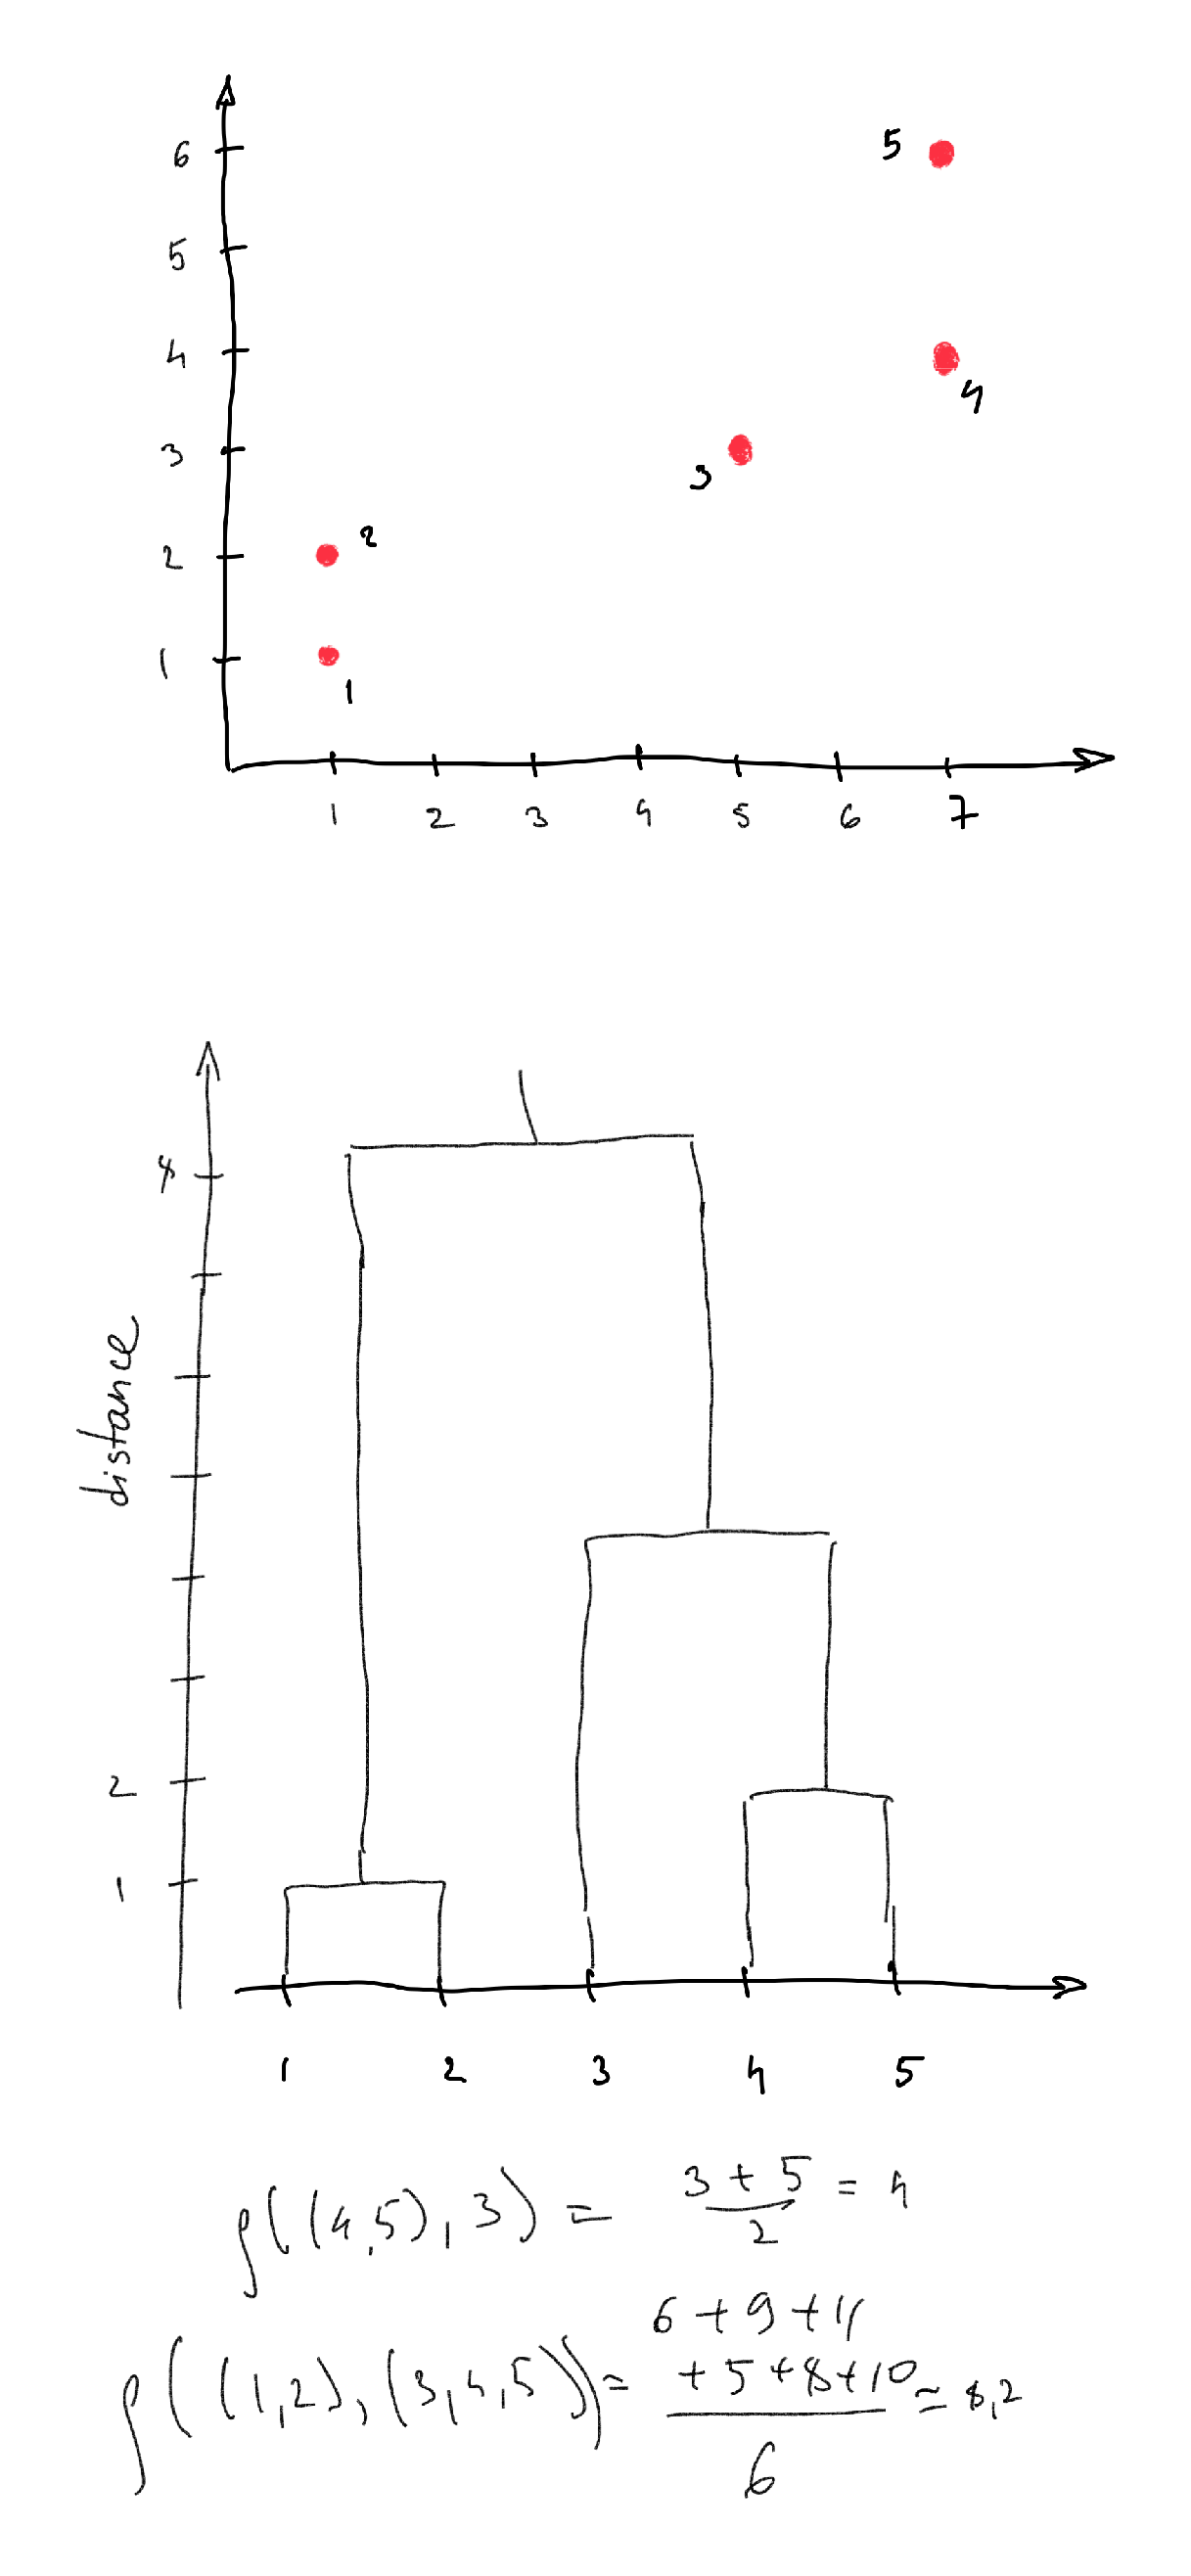
\includegraphics[width=1.1\columnwidth]{pics/dendrogram.pdf}
    %\caption{Движение $y$}
    \label{fig:boxplot}
\end{marginfigure}
Расстояния между кластерами могут быть заданы по разному и стоит обращать
внимание на решаемую задачу. Чтобы задать расстояние между кластерами надо
определить расстояние между точками и на ее основе определить метод построения
кластерного расстояния. Чаще всего используют такие методы:

\begin{itemize}
    \item среднее невзвешенное расстояние (average linkage clustering) -
        среднее расстояние между парами из различных кластеров

    \item центроид метод (устаревший) - расстояние между кластерами
        определяется как расстояние между центрами масс.

    \item метод дальнего соседа (complete linked clustering) - по расстоянию
        между максимально удаленными точками кластеров

    \item метод ближайшего соседа (single linkage clustering) - по расстоянию
        между самыми близкими точками

    \item метод Варда (Ward's method)
\end{itemize}

Дендрограмма выращивается снизу вверх. Сперва каждая точка представляет свой
собственный кластер. Если при достижении уровня $h$ расстояние между точками
равно $h$ то точки объединяются в один кластер (на рисунке это спайка). Процесс
повторяется до тех пор пока не останется один единственный кластер.

Для определения количества кластеров используют метод \emph{плеча}. Для этого
строится график где по оси абсцисс отмечаются шаги объединения (первое
объединение, второе и так далее), по оси ординат откладывается высота на
котором произошло объединение кластеров. На графике ищется точка перелома,
когда расстояние резко увеличивается. Это количество кластеров в данных по
методу локтя.
\marginpar{Результаты кластерного анализа нужно интерпретировать: анализ всегда
должен давать что-то новое о данных, что общего у объектов в кластере и чем
различаются кластеры.}
\marginpar{
    Кривую локтя можно построить и для метода k-средних. В этом случае по оси
    абсцисс будет лежать выбранный $k$ по оси ординат качество получившейся
    кластеризации.

    См. \fullcite{yandex:book}, глава 7.
}

Недостатки иерархической кластеризации:
\begin{itemize}
    \item Плохо справляется с данными которые вытянуты в длинные ленты в
        простраснтве

    \item Для вычисления требуется хранить попарные расстояния между объектами.
\end{itemize}

\section{DBSCAN}
Density-based spatial clustering of applications with noise. Сильный
топологический алгоритм. Основан на поиске связных компонент в покрытии данных
$\epsilon$-шарами. Количество кластеров определяет автоматически.

Все объекты в наблюдениях делятся на три категории:
\begin{itemize}
    \item core point (внутренние / основные) - если в окрестности есть более
        $N_0$ соседей

    \item border point (граничные) - если в окрестности меньше $N_0$ внутренних

    \item noise point (шумовые) - если в окрестности нет внутренних точек.
        Автоматически содержат меньше $N_0$ объектов.
\end{itemize}

Алгоритм DBSCAN:
\begin{marginfigure}
    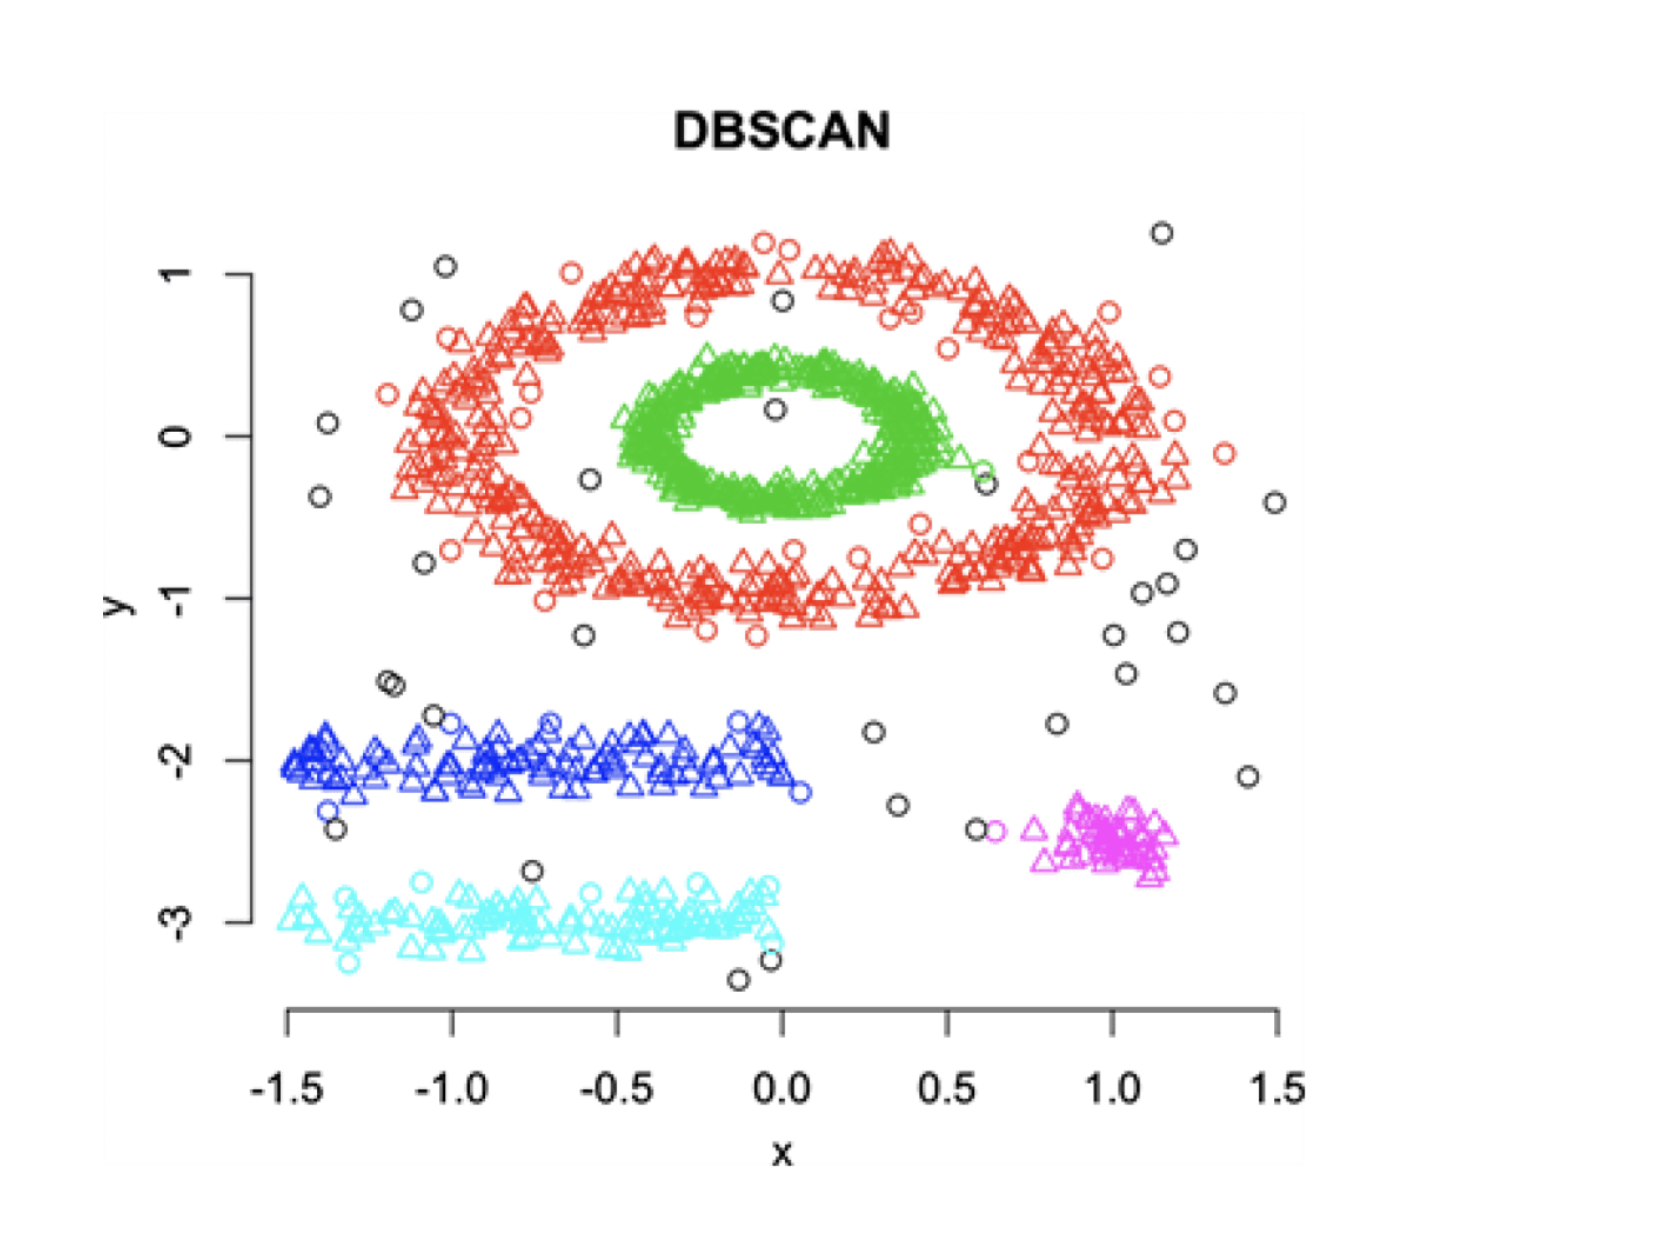
\includegraphics[width=1.3\columnwidth]{pics/dbscan.jpeg}
    %\caption{Движение $y$}
    \label{fig:boxplot}
\end{marginfigure}
\begin{enumerate}
    \item Шумовые точки удаляются из рассмотрения и не приписываются ни какому
        кластеру.

    \item Основные точки у которых есть общая окрестность соединяются ребром.
        Строится граф.

    \item В полученном графе вычисляются компоненты связности.

    \item Каждая граничная точка относится к тому кластеру, в который попала
        ближайшая к ней внутренняя точка.
\end{enumerate}

\chapter{Классификация и регрессия}

\section{Линейная регрессия}
\begin{marginfigure}
    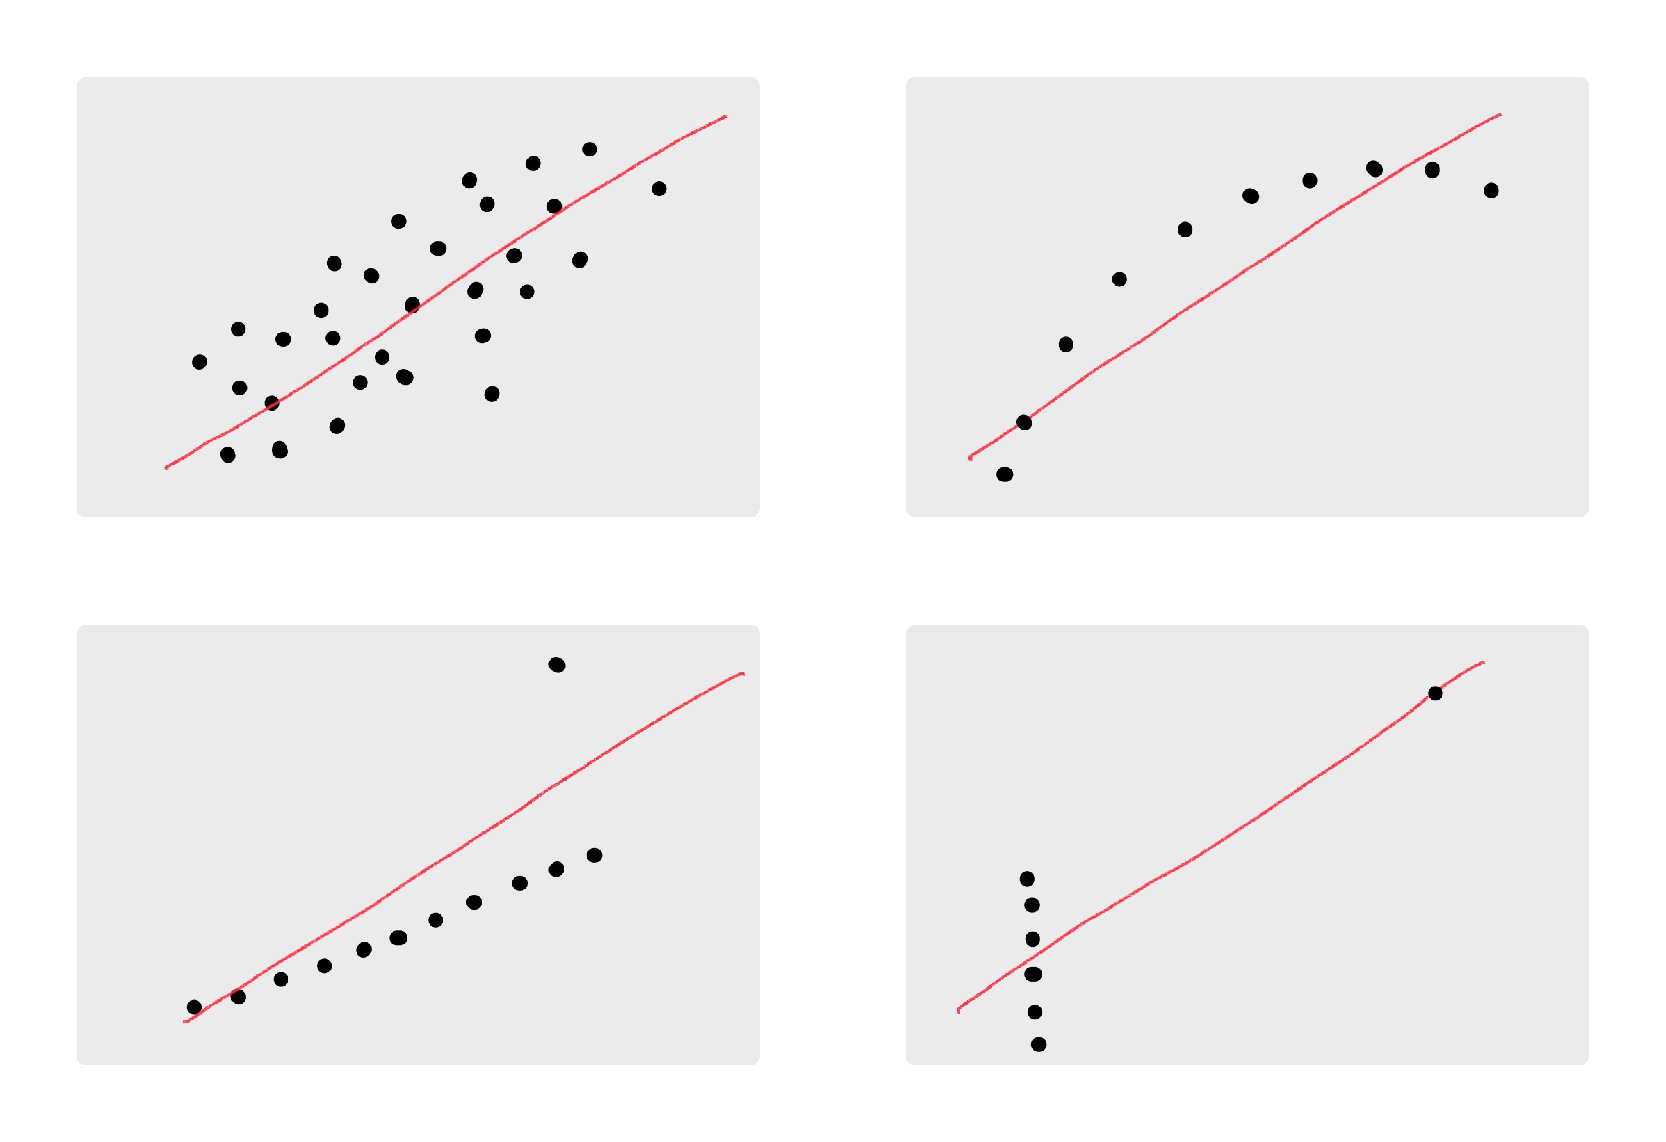
\includegraphics[width=1\columnwidth]{pics/anscombe_quartet.pdf}
    \caption{Квартет Анскомба. Иллюстрация как линейная регрессия может лажать. Для данных подобрали не ту модель или в данных есть сильные выбросы - все приводит к некорректному построению регрессии.}
    \label{fig:anscombe}
\end{marginfigure}

Для Определения на сколько модель хороша используют коэффициент детерминации. Чтобы его вычислить нужна обученная модель.
\begin{equation}
    \label{eq:coeff_of_determination}
    R^2 = 1 - \frac{D[y|x]}{D[y]}
\end{equation}
В сущностной части это на сколько дисперсия предсказания отличается от дисперсии наблюдений.

\marginpar{
    \emph{Наивная мультивариантная линейная регрессия:}
    \[ y = X\beta + \epsilon\]
    \[\epsilon \sim N(0,\, \sigma^2 I)\]
    $\epsilon$ - коэффициент \emph{невязки}, определяет шум системы.

    Коэффициенты находятся формулой
    \[ \hat \beta = (X^TX)^{-1}X^Ty \]

    Вариация вычисленных коэффициентов
    \[ Var(\hat \beta) = \sigma^2 (X^TX)^{-1}\]
    Это легко вывести если воспользоваться формулой дисперсии произведения 
    \[Var(AX) = A \cdot Var(X) \cdot A^T.\]
}

Во время построения модели регрессии самая большая проблема - наличие коллинеарных векторов (зависимых переменных в фичах). Чтобы очистить список фичей, можно проверить гипотезу что вычисленная фича нулевая (для каждой фичи индивидуально). 

\begin{equation*}
    \label{eq:zero_coeff_hyp}
    \left\{
    \begin{array}{lr}
        H_0: & \; \hat \beta_i = 0 \\
        H_1: & \; \hat \beta_i \ne 0
    \end{array}
    \right.
\end{equation*}

Если предположить что коэффициент имеет нормальное распределение, то мы можем
воспользоваться t-тестом Стьюдента и посчитать p-value. Если гипотеза не будет
отвергнута, это будет означать, что мы фичу стоит выкинуть потому что ее
коэффициент равен нулю. Соответственно там где гипотеза не подтвердилась фичи
являются ценными.

Выкидывать фичи стоит по одному. Начиная с самой слабой по p-value, каждый раз
с новым набором фичей анализ лучше проводить заново.\sidenote{\fullcite{Watts:ItS}}

\subsection{Для временных рядов}
Линейная регрессия может быть очень полезной во временных рядах, когда мы наблюдаем в них несколько сезонностей или когда данных относительно мало, нет нескольких полных сезонов в данных.

Чтобы учесть сезонность во временных рядах создают фичи:
\begin{itemize}
    \setlength\itemsep{0em}
    \item 1 - свободный коэффициент, bias
    \item $\delta_s(t)$ - учет сезонности, бинарный признак, что дата/время $t$ попало во временной интервал~$s$  (час, день, неделя, месяц и пр).
\end{itemize}
При этом очевидно, что если сложить все фичи $\delta_s(t)$ сезонности мы получим свободную переменную, то есть на лицо линейная зависимость. 

\section{Деревяшки (решающие деревья)}

\marginpar{
    {\bf Обозначения:}
    \begin{description}
        \item $N$ --- объем выборки
        \item $D$ --- размерность признаков
        \item $y = \{ y_i \}_{i=1}^N \subset \mathbb{R}^N$ --- вектор таргетов
        \item $X = \{x_i\}_{i=1}^N \in \mathbb{R}^{N \times D}$ --- матрица признаков
    \end{description}

    %\[x_{\text{строка}}^{\text{столбец}}\]
}

Решающее дерево имеет в узлах предикаты, а в листьях метки классов или другие значения в зависимости от задачи.

Чаще всего строят бинарные решающие деревья и используют такие предикаты:
\begin{equation}
    \label{eq:tree_predicat}
    B(x, j, t) = [x^j \le t] = B_{j,t}(x)
\end{equation}

\marginpar{
    \emph{Impurity criterion (критерий информативности)}~$H(R)$ оценивает
    качество распределения целевой переменной в множестве~$R$. 

    Поскольку это про оценку распределения часто используют энтропию или индекс
    Джини, но также может использоваться и квадрат/модуль ошибок и прочее.
}

Если в вершине выбрано какое-то разбиение и множество $R$ было разбито на два $R_l$ и $R_r$ то можно почитать на сколько мы сделали лучше этим разбиением.\sidenote{\fullcite{sokolov:desigion_tree}}
\begin{equation}
    \label{eq:tree_split_quality}
    Q(R, B_{j,t}) = H(R) - \frac{| R_l |}{| R | } H(R_l) - \frac{| R_r |}{| R |}H(R_r)
\end{equation}


Чтобы выбрать лучший вариант разбиения условия разбиения по признаку~$j$ можно
упорядочить все наблюдения в узле по этому признаку постепенно перебрать все
варианты разбиений и выбрать тот в котором функция качества~$Q$ достигает
максимума. Эту процедуру повторяем для всех $j = \overline{1, D}$ и выбираем лучшее разбиение.

\begin{equation}
    \label{eq:opt_node_value}
    (j_{opt}, t_{opt}) = \argmax_{j, t} Q(R, B_{j,t})
\end{equation}

\marginpar{Если на тестовой выборке результат заметно хуже, а мы очень хотим обучить дерево, можно попробовать упростить модель, сильнее ограничить глубину дерева.}

\marginpar{
    Для решения \emph{задачи регрессии} достаточно подобрать критерий
    информативности. Например, это может быть квадрат отклонения от среднего

    \[
        H(R) = \frac{1}{|R|} \sum_{(x_i,\,y_i) \in R}
        \left(
            y_i - \frac{1}{|R|} \sum_{(x_i,\,y_i) \in R} y_i
        \right)^2
    \]
}

Для процедуры критерий останова можно вводить разными способами. Самые
популярные такие:
\begin{itemize}
    \setlength\itemsep{0em}
    \item максимальная глубина дерева,
    \item максимальное количество листьев,
    \item минимальное число объектов в листе,
    \item все объекты в листе лежат в одном классе,
    \item качество улучшилось не более чем на $x$ процентов.
\end{itemize}

Деревья дают кусочно-линейные решения, однако у них есть преимущества в том,
что они могут вытащить нелинейные зависимости; а также и недостатки, за
пределами наблюдений регрессия будет предсказываться константой. Другими
словами регрессия на деревьях не умеет экстраполировать, зато может быть
полезна в интерполяции.

\medskip
\printbibliography

\end{document}
